\documentclass[15pt]{article}

% Language setting
% Replace `english' with e.g. `spanish' to change the document language
\usepackage[english]{babel}

% Set page size and margins
% Replace `letterpaper' with `a4paper' for UK/EU standard size
\usepackage[letterpaper,top=2cm,bottom=2cm,left=3cm,right=3cm,marginparwidth=1.75cm]{geometry}

% Useful packages
\usepackage{amsmath}
\usepackage{graphicx}
\usepackage[colorlinks=true, allcolors=blue]{hyperref}
\usepackage{listings}
\usepackage{color}

\definecolor{dkgreen}{rgb}{0,0.6,0}
\definecolor{gray}{rgb}{0.5,0.5,0.5}
\definecolor{mauve}{rgb}{0.58,0,0.82}

\lstset{frame=tb,
  language=C++,
  aboveskip=3mm,
  belowskip=3mm,
  showstringspaces=false,
  columns=flexible,
  basicstyle={\small\ttfamily},
  numbers=none,
  numberstyle=\tiny\color{gray},
  keywordstyle=\color{blue},
  commentstyle=\color{dkgreen},
  stringstyle=\color{mauve},
  breaklines=true,
  breakatwhitespace=true,
  tabsize=3
}

\title{Counting Flags}
\author{Timothy Gao}
\date{}

\begin{document}

\maketitle

You are given a $N$ $(1 \leq N \leq 1000)$ by $M$ $(1 \leq M \leq 1000)$ grid of binary 0/1 values. Define a "flag" as an isosceles right triangle where the 90$^{\circ}$ vertex is the right-most and bottom-most element. Examples:

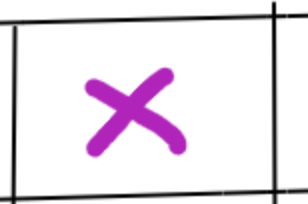
\includegraphics[width=0.2\textwidth]{1.png}
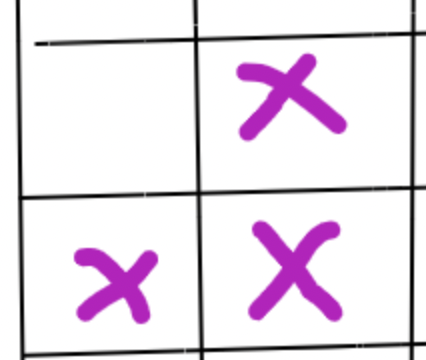
\includegraphics[width=0.2\textwidth]{2leg.png}
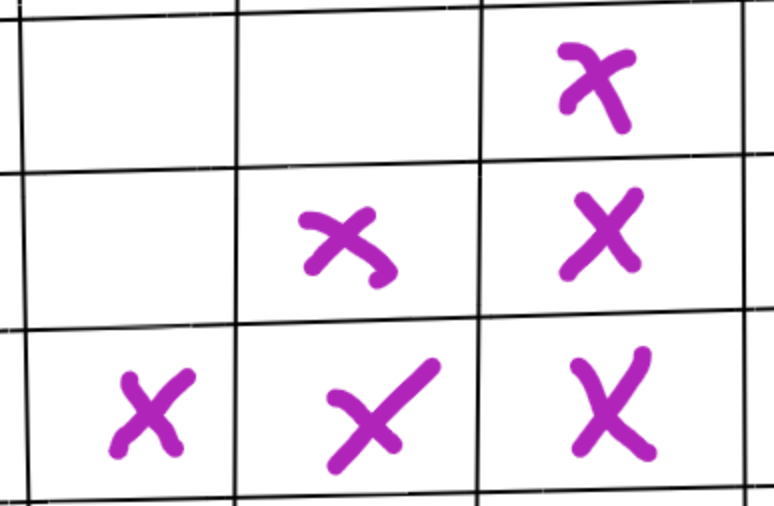
\includegraphics[width=0.2\textwidth]{3leg.png}
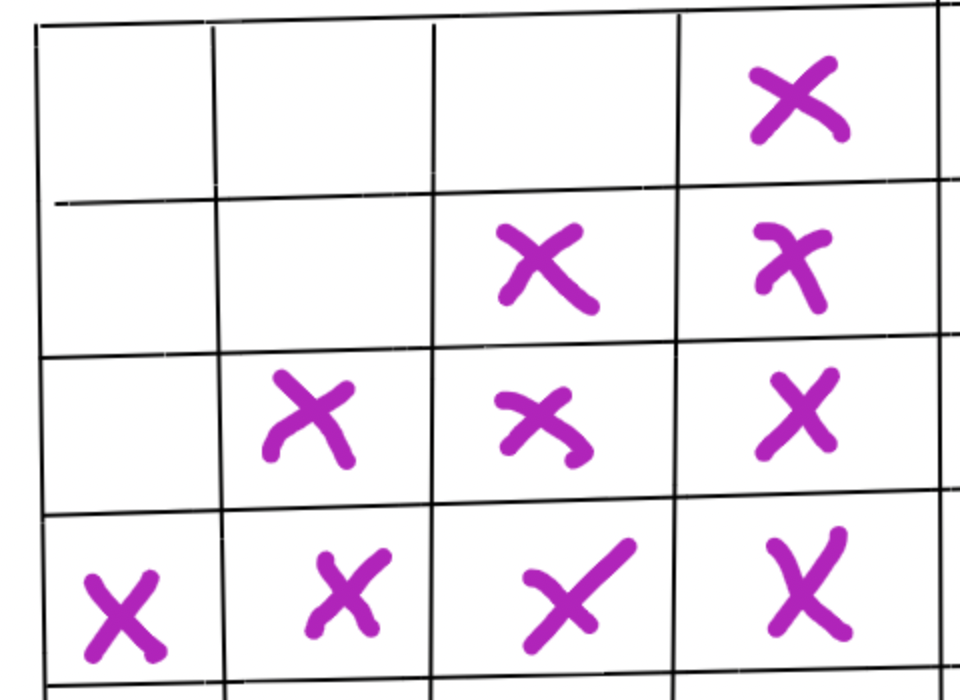
\includegraphics[width=0.2\textwidth]{4leg.png}
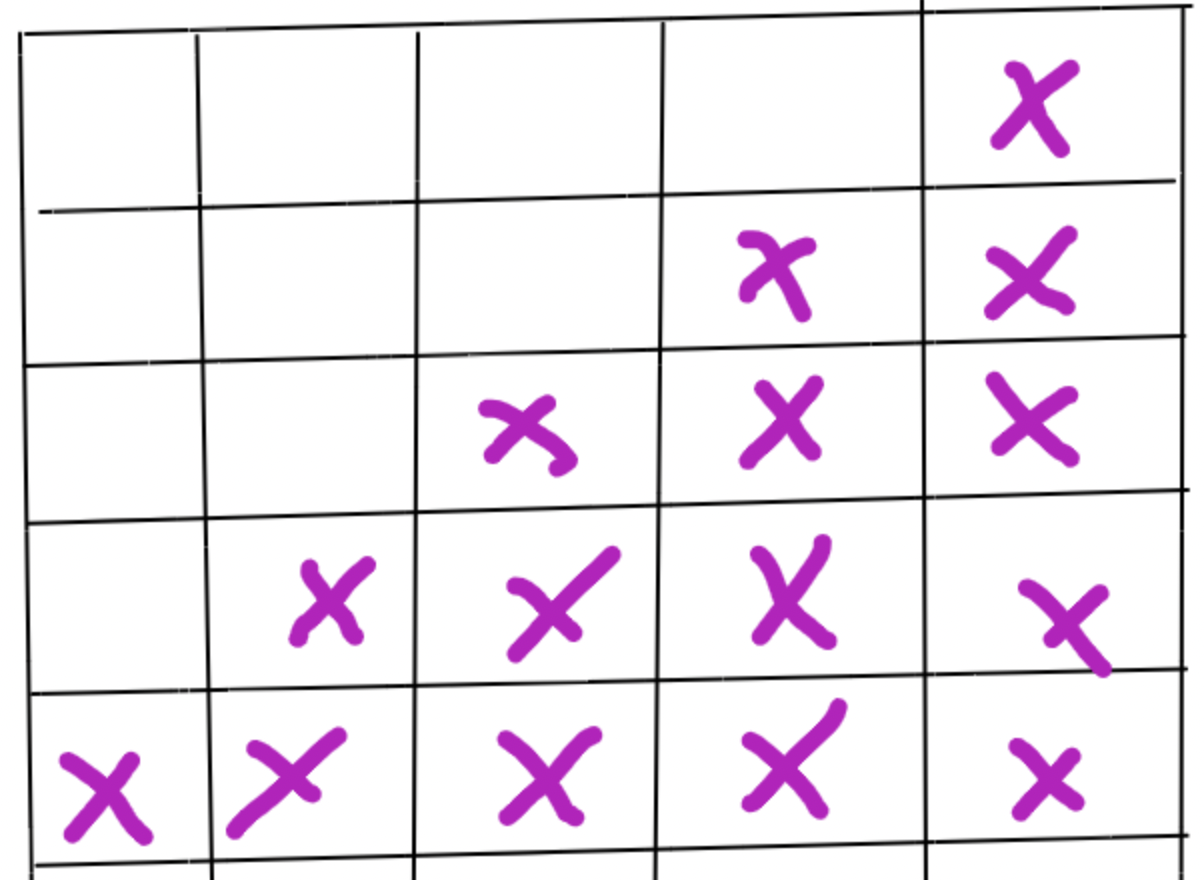
\includegraphics[width=0.2\textwidth]{5leg.png}

Count the number of flags fully filled by 1s in the grid.

\section{Initial Observations}

Define angle point as the cell where two legs of the flag intersect (i.e., the 90$^{\circ}$ vertex).

Let's start with a brute force solution. We iterate over all angle points, trying all leg lengths $0...N$, then for each length we verify in $N^2$ whether the right triangle made by the angle flag and leg length is entirely filled by 1s. This runs for $\mathcal{O}(N^5)$, but it's a good starting point.

One way we to optimize this brute force solution is by noticing that as we iterate through the lengths, we don't need to scan the entire area but only the new cells added. 

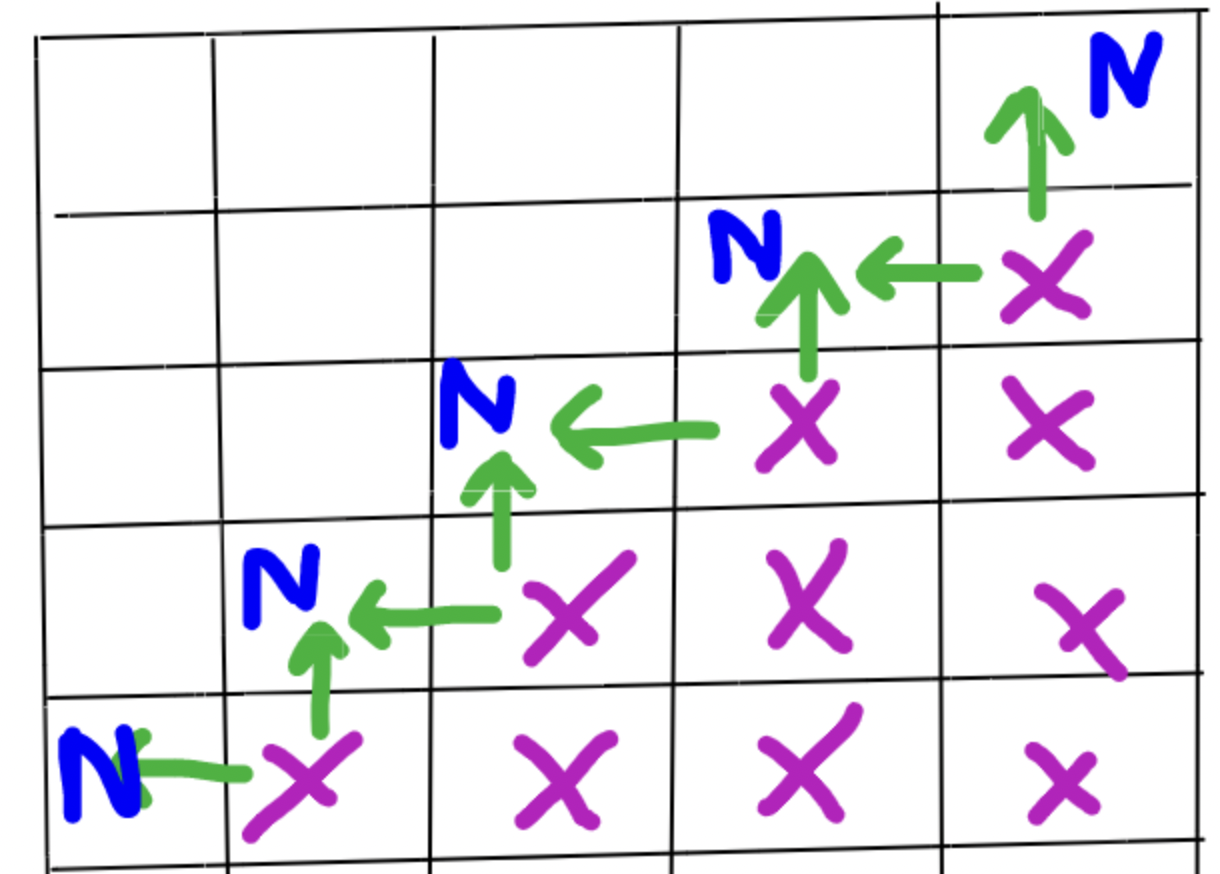
\includegraphics[width=1\textwidth]{bluenew.png}

With this, each new length takes $\mathcal{O}(N)$ rather than $\mathcal{O}(N^2)$ to verify, allowing us to optimize our brute force down to $\mathcal{O}(N^4)$. The key idea here is that instead of counting all cells for each new angle point and length, we can utilize the results of our previous length and only count at most $N$ new cells. Let's see how we can extend this idea of "building on previous results" further.

Rather than counting all possible flags in the grid, we can simply count the largest possible flag that can be made with angle point starting at each cell. If the largest flag has side length $x$, then all triangles with lengths $1...x-1$ also exist at the same angle point. We create an array $A$ and increment $A[x]$++ for the largest flag at every cell. Afterwards, we take the suffix sums of $A$, i.e. $A[i]$ += $A[i+1]$ to find the number of flags with every leg length $i$.

\section{Arriving at the Solution}

This idea of "building on previous solutions" inspires us to think in terms of dynamic programming. Let dp[i][j] be the side length of the largest flag with angle point $(i, j)$. We can in fact directly utilize other dp values. Consider the state transition

\[
dp[i][j] = min(dp[i-1][j], dp[i][j-1]) + 1
\]

This is best explained visually: 

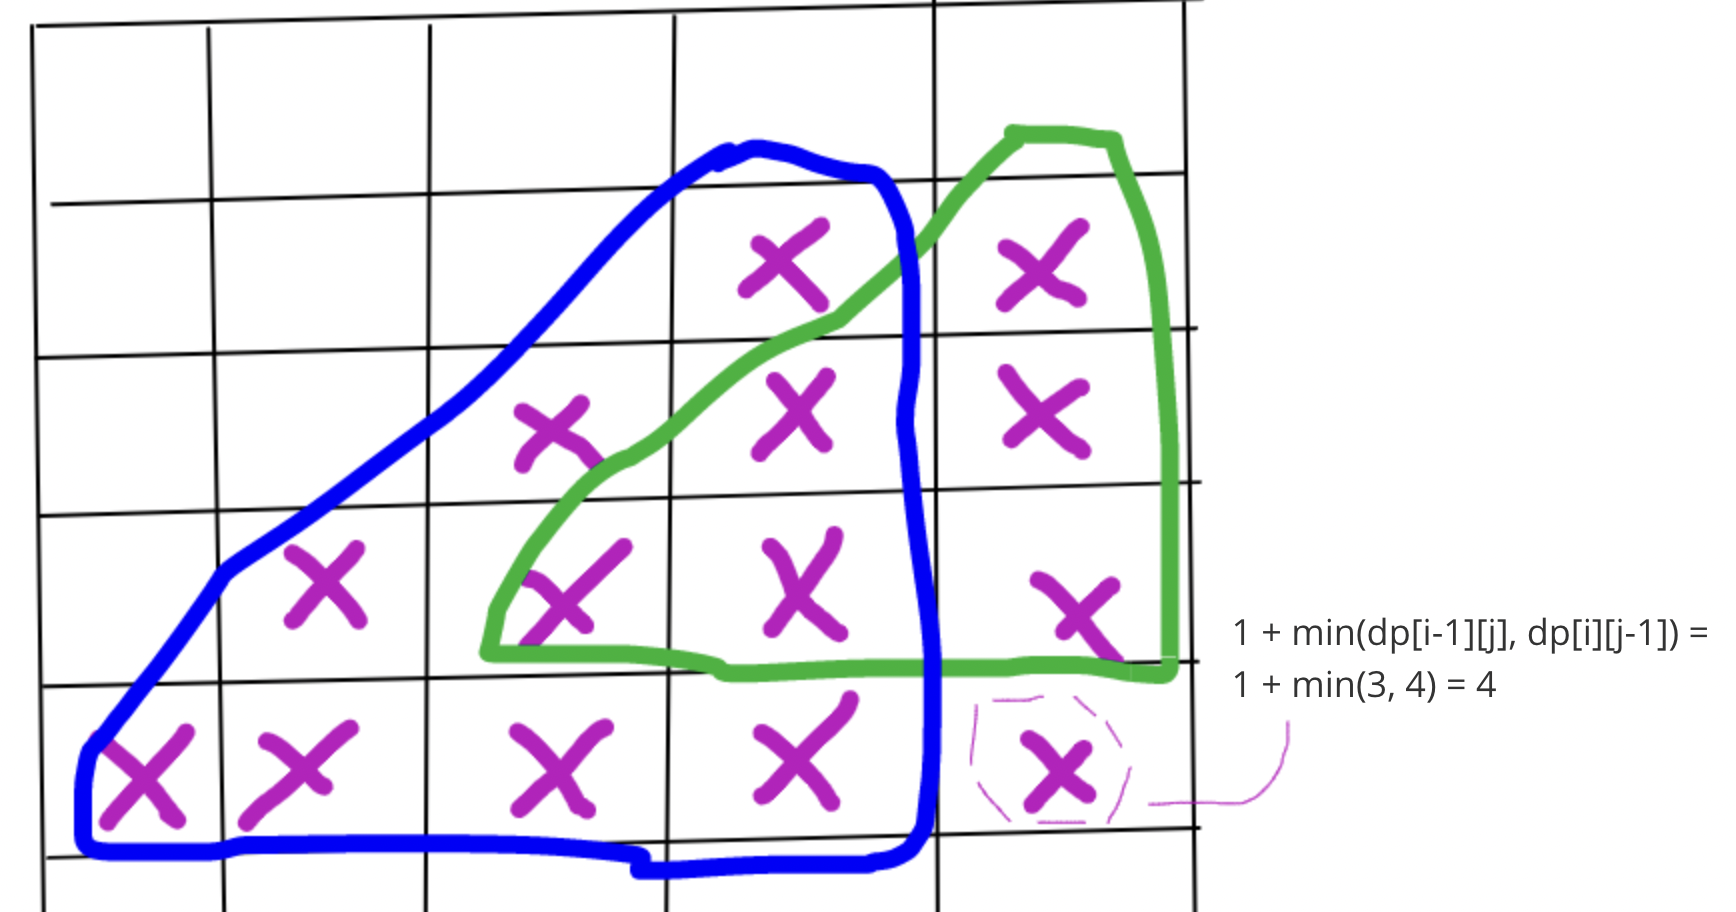
\includegraphics[width=1\textwidth]{dpexplained.png}

Notice that we can "construct" a right triangle at the current cell $(i, j)$ by taking advantage of previously known results of the largest flag at $(i-1, j)$ and $(i, j-1)$. And more specifically, the maximum leg length of the current cell is limited by the smaller of the two.

Computing this DP takes $\mathcal{O}(NM)$ as each of the $N \cdot M$ states need to be visited only once. My code is implemented with bottom-up, but top-down DP is also comfortably fast enough.

Using the suffix sums idea we conceived of earlier, we can then compute all leg lengths in a post-processing $\mathcal{O}(N)$, leading to a final linear time complexity of $\mathcal{O}(NM)$.

Note: An alternate solution exists for this problem utilizing a similar approach to \href{https://leetcode.com/problems/largest-rectangle-in-histogram/}{The Largest Rectangle Problem}, by employing binary search or prefix sums on each row as we iterate down. This adds a log factor but can still pass under the time limit with some constant factor optimization.

\section{Code}
\begin{lstlisting}
//@timothyg

#include <bits/stdc++.h>
 
using namespace std;
 
typedef long long ll;
typedef pair<int, int> pii;

#define pb push_back

#define f first
#define s second

const int maxn = 1005;
int matrix[maxn][maxn];
int dp[maxn][maxn];
int triangle[maxn];

int main(){
    ios_base::sync_with_stdio(false); cin.tie(0);
    
    int N, M; cin >> N >> M;
    for(int i = 0; i<N; i++){
        for(int j = 0; j<M; j++){
            cin >> matrix[i][j];
        }
    }

    //dp[i][j] = min(dp[i-1][j], dp[i][j-1]) + 1
    for(int i = 0; i<N; i++){
        for(int j = 0; j<M; j++){
            if(matrix[i][j] == 0) continue;
            dp[i][j] = min(
                i == 0 ? 0 : matrix[i-1][j],    
                j == 0 ? 0 : matrix[i][j-1]
            );  
            dp[i][j]++;
            triangle[dp[i][j]]++;
        }
    }
    
    //suffix sums
    for(int i = max(N, M)-1; i>=0; i--){
        triangle[i] += triangle[i+1];
    }
    
    int Q; cin >> Q;
    while(Q--){
        int x; cin >> x;
        cout << triangle[x] << '\n';
    }

    return 0;
}
\end{lstlisting}
\end{document}